% questions.tex —— 2004 年·普通高等学校春季招生考试·安徽卷文科 · 题目内容片段（无答案）
% 由 tools/generate_projects.py 依来源总账自 2004/2004_数学真题_春季安徽文_试题.md 生成，勿手改（改源 MD 后重跑）


\gkpart{数学试卷}

\begin{gktip}
\textbf{来源说明}：本稿依固定来源 PDF 转录，先以文字层定位，再逐页目视核对。文件共 2 页，版面为 A3，印刷页码 151–152；PDF 元数据表明其由 XeTeX 生成，因此不称为原始扫描件。上游出版物、出版者及版次尚未核实；来源清单中的 \texttt{ready} 只表示该文件可用。当前 \texttt{paper_id=gk-2004-spring-anhui-arts} 的 canonical 关系仅表示本库将该固定副本绑定为题面来源，不认证官方来源身份。原题条件与选项按文件保留；第 8 题系数根号已依据页图确认，不能仅依赖文字层抽取结果。

\textbf{答案说明}：固定 PDF 未含答案页；本稿不补录官方答案，也不将本项目的推导答案冒充官方答案。\texttt{official_answer} 保持 \texttt{null}。

\textbf{图表说明}：第 20 题三棱柱图已另绘为 TikZ 矢量示意，保留原图的线段拓扑和 \texttt{AC} 虚线；不声称按比例，未将源页 PNG/JPEG 入库。详见图表清单。
\end{gktip}

\gkpart{一、选择题}

\begin{question}
\gkti{1}若集合 $M=\{-1,0,1,2\}$，$N=\{x\mid x(x-1)=0\}$，则 $M\cap N=$\mbox{（　　）}。

（A）$\{-1,0,1,2\}$　　（B）$\{0,1,2\}$　　（C）$\{-1,0,1\}$　　（D）$\{0,1\}$

\end{question}
\begin{question}
\gkti{2}不等式 $|2x^2-1|\leq 1$ 的解集为\mbox{（　　）}。

（A）$\{x\mid -1\leq x\leq 1\}$　　（B）$\{x\mid -2\leq x\leq 2\}$

（C）$\{x\mid 0\leq x\leq 2\}$　　（D）$\{x\mid -2\leq x\leq 0\}$

\end{question}
\begin{question}
\gkti{3}已知 $F_1,F_2$ 为椭圆 $\dfrac{x^2}{a^2}+\dfrac{y^2}{b^2}=1\ (a>b>0)$ 的焦点，$M$ 为椭圆上一点，$MF_1$ 垂直于 $x$ 轴，且 $\angle F_1MF_2=60^\circ$，则椭圆的离心率为\mbox{（　　）}。

（A）$\dfrac{1}{2}$　　（B）$\dfrac{\sqrt{2}}{2}$　　（C）$\dfrac{\sqrt{3}}{3}$　　（D）$\dfrac{\sqrt{3}}{2}$

\end{question}
\begin{question}
\gkti{4}已知向量 $\vec a=(1,2)$，$\vec b=(2,3)$，$\vec c=(3,4)$，且 $\vec c=\lambda_1\vec a+\lambda_2\vec b$，则 $\lambda_1,\lambda_2$ 的值分别是\mbox{（　　）}。

（A）$-2,1$　　（B）$1,-2$　　（C）$2,-1$　　（D）$-1,2$

\end{question}
\begin{question}
\gkti{5}等边三角形 $ABC$ 的边长为 $4$，$M,N$ 分别为 $AB,AC$ 的中点，沿 $MN$ 将 $\triangle AMN$ 折起，使得面 $AMN$ 与面 $MNCB$ 所处的二面角为 $30^\circ$，则四棱锥 $A-MNCB$ 的体积为\mbox{（　　）}。

（A）$\dfrac{3}{2}$　　（B）$\dfrac{\sqrt{3}}{2}$　　（C）$\sqrt{3}$　　（D）$3$

\end{question}
\begin{question}
\gkti{6}已知数列 $\{a_n\}$ 满足 $a_0=1$，$a_n=a_0+a_1+\cdots+a_{n-1}\ (n\geq 1)$，则当 $n\geq 1$ 时，$a_n=$\mbox{（　　）}。

（A）$2^n$　　（B）$\dfrac{n(n+1)}{2}$　　（C）$2^{n-1}$　　（D）$2^n-1$

\end{question}
\begin{question}
\gkti{7}若二面角 $\alpha-l-\beta$ 为 $120^\circ$，直线 $m\perp\alpha$，则 $\beta$ 所在平面内的直线与 $m$ 所成角的取值范围是\mbox{（　　）}。

（A）$(0^\circ,90^\circ]$　　（B）$[30^\circ,60^\circ]$　　（C）$[60^\circ,90^\circ]$　　（D）$[30^\circ,90^\circ]$

\end{question}
\begin{question}
\gkti{8}若 $\sin 2\alpha=\dfrac{24}{25}$，则 $\sqrt{2}\cos\left(\dfrac{\pi}{4}-\alpha\right)$ 的值为\mbox{（　　）}。

（A）$\dfrac{1}{5}$　　（B）$\dfrac{7}{5}$　　（C）$\pm\dfrac{1}{5}$　　（D）$\pm\dfrac{7}{5}$

\end{question}
\begin{question}
\gkti{9}直角坐标 $xOy$ 平面上，平行直线 $x=n\ (n=0,1,2,\ldots,5)$ 与平行直线 $y=n\ (n=0,1,2,\ldots,5)$ 组成的图形中，矩形共有\mbox{（　　）}。

（A）$25$ 个　　（B）$36$ 个　　（C）$100$ 个　　（D）$225$ 个

\end{question}
\begin{question}
\gkti{10}若直线 $ax+y=1$ 与圆 $(x-\sqrt{3})^2+(y-2)^2=1$ 有两个不同的交点，则 $a$ 的取值范围是\mbox{（　　）}。

（A）$(1,\sqrt{3})$　　（B）$(-\sqrt{3},0)$　　（C）$(\sqrt{3},+\infty)$　　（D）$(-\infty,-\sqrt{3})$

\end{question}
\begin{question}
\gkti{11}若 $f(\sin x)=2-\cos 2x$，则 $f(\cos x)=$\mbox{（　　）}。

（A）$2-\sin 2x$　　（B）$2+\sin 2x$　　（C）$2-\cos 2x$　　（D）$2+\cos 2x$

\end{question}
\begin{question}
\gkti{12}已知直线 $l:x-y-1=0$，$l_1:2x-y-2=0$。若直线 $l_2$ 与 $l_1$ 关于 $l$ 对称，则 $l_2$ 的方程是\mbox{（　　）}。

（A）$x-2y+1=0$　　（B）$x-2y-1=0$　　（C）$x+y-1=0$　　（D）$x+2y-1=0$

\end{question}
\gkpart{二、填空题}

\begin{question}
\gkti{13}抛物线 $y^2=6x$ 的准线方程为 $\underline{\qquad\qquad}$。

\end{question}
\begin{question}
\gkti{14}在 $5$ 名学生（$3$ 名男生，$2$ 名女生）中安排 $2$ 名学生值日，其中至少有 $1$ 名女生的概率是 $\underline{\qquad\qquad}$。

\end{question}
\begin{question}
\gkti{15}函数 $y=x-x^2\ (x\in\mathbb{R})$ 的最大值为 $\underline{\qquad\qquad}$。

\end{question}
\begin{question}
\gkti{16}若 $\left(x+\frac{1}{x}-2\right)^n$ 的展开式中常数项为 $-20$，则自然数 $n=$ $\underline{\qquad\qquad}$。

\end{question}
\gkpart{三、解答题}

\begin{question}
\gkti{17}解关于 $x$ 的不等式：$\log_a^{2}x<2\log_ax\ (a>0\text{ \text{且} }a\neq 1)$。

\end{question}
\begin{question}
\gkti{18}已知数列 $\{b_n\}$ 的首项 $b_1=1$。其前 $n$ 项和 $B_n=\dfrac{1}{4}(b_n+1)^2$，求 $\{b_n\}$ 的通项公式。

\end{question}
\begin{question}
\gkti{19}已知 $k>0$，直线 $l_1:y=kx$，$l_2:y=-kx$。

(1) 证明：到 $l_1,l_2$ 的距离的平方和为定值 $a\ (a>0)$ 的点的轨迹是圆或椭圆；

(2) 求到 $l_1,l_2$ 的距离之和为定值 $c\ (c>0)$ 的点的轨迹。

\Needspace{0.4\textheight}
\end{question}
\begin{question}
\gkti{20}已知三棱柱 $ABC-A_1B_1C_1$ 中，底面边长和侧棱长均为 $a$，侧面 $A_1ACC_1\perp$ 底面 $ABC$，$A_1B=\frac{\sqrt{6}}{2}a$。

(1) 求异面直线 $AC$ 与 $BC_1$ 所成角的余弦值；

(2) 求证：$A_1B\perp$ 面 $AB_1C$。
\nopagebreak[4]
\begin{center}% 2004 年春季安徽文科卷第 20 题：三棱柱示意图；not to scale.
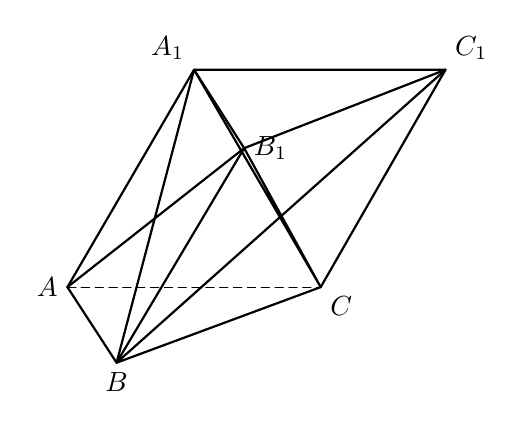
\begin{tikzpicture}[line cap=round,line join=round,scale=1.2]
  \coordinate (A) at (0,0);
  \coordinate (B) at (0.52,-0.80);
  \coordinate (C) at (2.68,0);
  \coordinate (A1) at (1.34,2.30);
  \coordinate (B1) at (1.87,1.47);
  \coordinate (C1) at (4.00,2.30);

  % Hidden base edge in the source drawing.
  \draw[densely dashed] (A) -- (C);
  % Triangular bases and corresponding lateral edges.
  \draw[thick] (A) -- (B) -- (C);
  \draw[thick] (A1) -- (B1) -- (C1) -- cycle;
  \draw[thick] (A) -- (A1) (B) -- (B1) (C) -- (C1);
  % Construction lines shown in the source figure for the two subquestions.
  \draw[thick] (A1) -- (B) (A1) -- (C) (A) -- (B1) (B1) -- (C) (B) -- (C1);

  \node[left] at (A) {$A$};
  \node[below] at (B) {$B$};
  \node[below right] at (C) {$C$};
  \node[above left] at (A1) {$A_1$};
  \node[right] at (B1) {$B_1$};
  \node[above right] at (C1) {$C_1$};
\end{tikzpicture}
\end{center}
\nopagebreak[4]
\end{question}
\begin{question}
\gkti{21}某商场从生产厂家以每件 $20$ 元购进一批商品，若该商品零售价定为 $p$ 元，则销售量 $Q$（单位：件）与零售价 $p$（单位：元）有如下关系：

\nopagebreak[4]
\[
Q=8300-170p-p^2.
\]

问该商品零售价定为多少时毛利润 $L$ 最大，并求出最大毛利润。（毛利润 $=$ 销售收入 $-$ 进货支出。）

\end{question}
\begin{question}
\gkti{22}已知抛物线 $C:y=x^2+4x+\frac{7}{2}$，过 $C$ 上一点 $M$，且与 $M$ 处的切线垂直的直线称为 $C$ 在点 $M$ 的法线。

(1) 若 $C$ 在点 $M$ 的法线的斜率为 $-\dfrac{1}{2}$，求点 $M$ 的坐标 $(x_0,y_0)$；

(2) 设 $P(-2,a)$ 为 $C$ 对称轴上的一点，在 $C$ 上是否存在点，使得 $C$ 在该点的法线通过点 $P$？若有，求出这些点，以及 $C$ 在这些点的法线方程；若没有，请说明理由。

\end{question}